\section{Auswertung}
\label{sec:Auswertung}



\subsection{Bestimmung der Metalle über die Dichte}
Die Metalle lassen sich über ihr Volumen V und ihre Masse m bestimmen(Tab.1).
Im Vergleich zu dem Literaturwert von Messing mit $8.41\, \frac{g}{cm^3}$\cite{litval}
zeigt sich, dass beide Stäbe aus Messing bestehen.
\begin{table}[h]
  \centering
  \label{tab:lit}
  \begin{tabular}{ c c c c c c }
    \toprule
    {$\text{Stab}$}
   &{$l \,\, \text{in} \, [m]$}
   &{$d \,\, \text{in} \, [m]$}
   %&{$h \, in \, [m]$}
   &{$V \,\, \text{in} \, [m^3]$}
   &{$m \,\, \text{in} \, [kg]$}
   &{$\rho \,\, \text{in} \, [\frac{g}{cm^3}]$} \\
    \midrule
     {$\text{eckig}$}&60&1&60&502.4 & 8.367 \\
     {$\text{rund}$}&60.05&1&15$\pi$&394.4 & 8.361 \\
    \bottomrule
  \end{tabular}
  \caption{Dichte der Metalle}
\end{table}


\subsection{Eckiger Stab, einseitige Einspannung}

Über die Differenz der Auslenkung  ergibt sich nach
$D(x) = D_0 - D_m$. Die Einspannlänge beträgt $L_1 = 0.493m$ und
das verwendete Gewicht $m_1 = 1.1932 kg$.

\begin{table}[h]
  \centering
  \label{tab:lit2}
  \begin{tabular}{ c c c }
    \toprule
    $x \,\, \text{in} \, [mm]$
   &{$D(x) \,\, \text{in} \, [mm]$}
   &{$(Lx^2- \frac{x^3}{3}) \,\, \text{in} \, [mm^3]$} \\

    \midrule
     0 & 0 & 0 \\
     0 & 0 & 0 \\
    \bottomrule
  \end{tabular}
  \caption{Dichte der Metalle}
\end{table}

\begin{figure}[h]
  \centering
  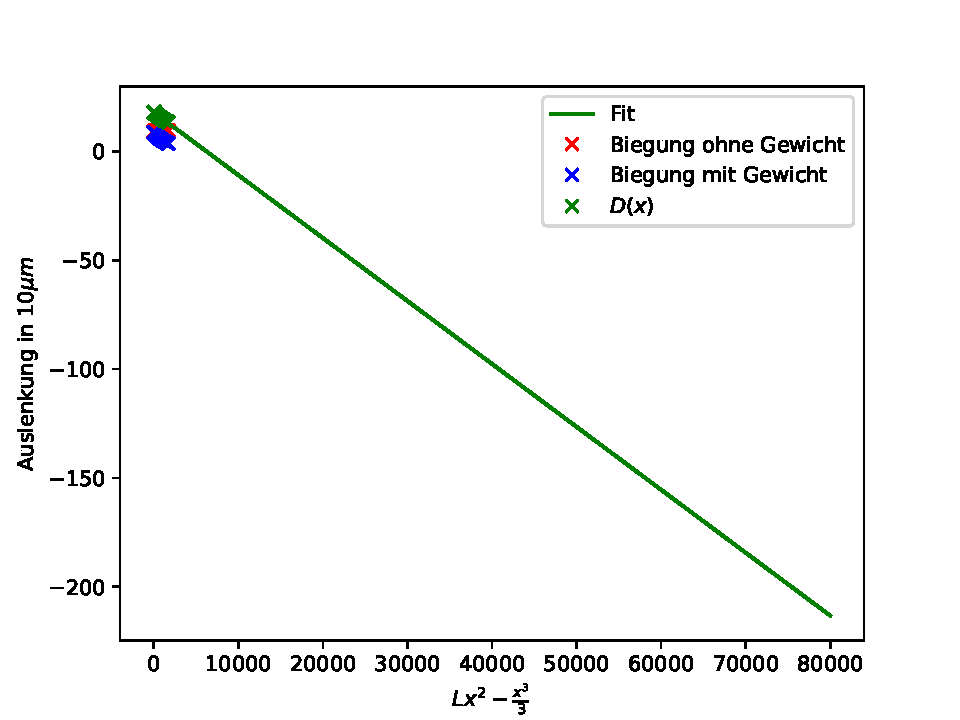
\includegraphics{build/plot1.pdf}
  \caption{Eckiger Stab, einseitige Einspannung}
  \label{fig:plot1}
\end{figure}



Mit Hilfe von Python wurde eine Regressiongerade berechnet (Abb.3).
Hierbei wird $(Lx^2- \frac{x^3}{3})$ auf der x-Achse gegen $D(x)$ auf der y-Achse
gesetzt, woraus sich die Werte
\begin{align*}
  a &= \SI{8.15(104)e-5}{\per\square\meter} \\
  b &= \SI{7.8205(257)e-2}{\meter} \\
\end{align*}
für die Regressionsgerade ergeben.
\newline
Das vorliegende Trägheitsmoment ist
\begin{equation*}
  I = 1.667* 10^{-9}\, m^4.
\end{equation*}

Hiermit wird der Elastizitätsmodul nach \ref{eqn:einseitig} bestimmt.

\begin{equation*}
  E = \SI{1.20(15)e+5}{\newton\per\square\meter}
\end{equation*}






\subsection{Runder Stab, einseitige Einspannung}
Die Einspannlänge beträgt 
\begin{figure}[h]
  \centering
  \includegraphics{build/plot2.pdf}
  \caption{Plot2.}
  \label{fig:plot2}
\end{figure}

\subsection{Runder Stab, beidseitige Einspannung}
\begin{figure}
  \centering
  \includegraphics{build/plot3.pdf}
  \caption{Plot3.}
  \label{fig:plot3}
\end{figure}
